\setsection{Améliorations notables : fausses alertes et outils de mesure}
	Comme nous l'avons vue précédement (section 3) le problème de fusion de chaîne a amené a créé les \glspl{rainbow}. Mais il se peut aussi qu'il y ait collision entre la chaîne que nous générons et une des chaînes des tables. Lorsque ce cas arrive nous parlons de fausse alertes.
	De plus jusqu'à présent nous n'avons pas réellement présenté d'outils permettant de comparer les efficacités des différentes méthodes de compromis.

\setsubsection{Points de contrôles}
	Afin de vérifier que 2 chaînes ne fusionnent il a été proposé par \cite{checkpoints} d'instaurer des points de contrôles. Pour ce faire $\alpha_i$ positions sont fixées. Pour chaque chaîne, la fonction G est évaluée et la valeur est stockée, à chacune de ces positions. Lors de la génération de la chaîne $Y_1,Y_2,...,Y_s$ nous évaluons également les $G(Y_{\alpha_i+s-t})$. La moindre différence entre les points de contrôles de cette chaîne et celle de la table correspond à une fausse alerte.

\begin{figure}
	\begin{minipage}{.5\textwidth}
		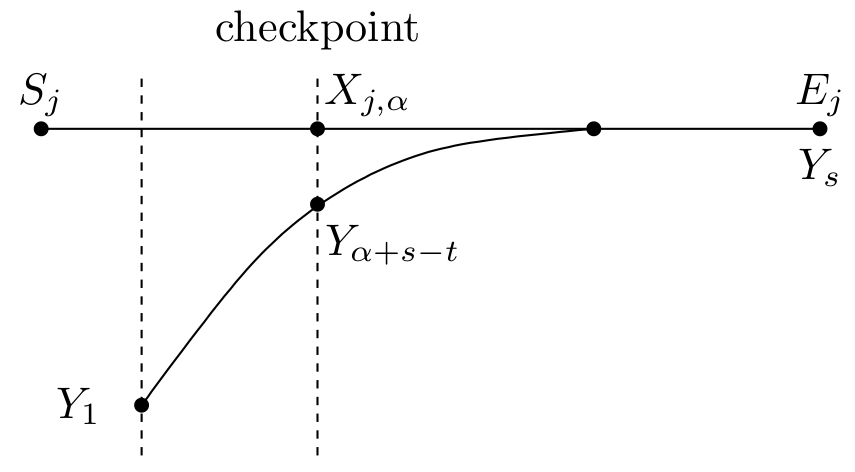
\includegraphics[width=0.9\linewidth]{other/FalseAlarmDetected.png}
		%\captionof{figure}{Fausse alerte détecté avec une probabilité de 1/2}
	\end{minipage}
	\begin{minipage}{.5\textwidth}
	    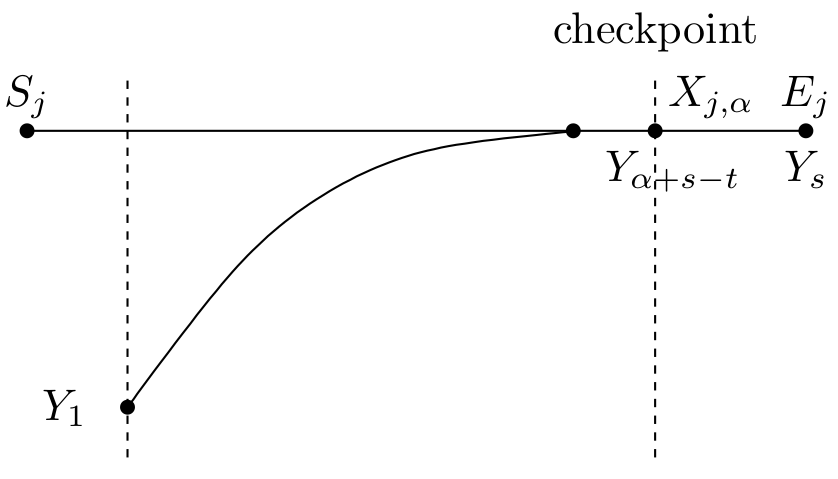
\includegraphics[width=0.9\linewidth]{other/FalseAlarmNotDetected.png}
		%\caption{Fausse alerte non détecté}
  	\end{minipage}
\end{figure}

	\bigskip
	
	les points de contrôle doivent être simple à évaluer et stocker, il est considéré que g sort les bits les moins significatifs. nous estimons selon la formule suivante la détection d'une fausse alerte :
\begin{align*}
pr\{g(x_{j,\alpha}) \neq g(y_{\alpha +s-t}) \mid x_{j,a} \neq y_{\alpha+s-t}\}=\frac{1}{2}(1-\frac{1}{2^{\mid k \mid}}) \approx \frac{1}{2}
\end{align*}




\setsubsection{Outils de comparaison}
	

\setsubsection{Conclusion}


\endinput{}
